\section{Testing}
In diesem Kapitel ist das Testing der Applikation beschrieben. Auf Unit-Tests wurde verzichtet, da ohne aufwendiges Refactoring der bestehende Code sehr schwierig zu testen ist. Stattdessen werden Integrationstests verwendet, um das Zusammenspiel der Klassen über die verschiedenen Softwareschichten zu testen.

\subsubsection{Verwendete Libraries}
Für die Tests wurde neben Junit auch die Libraries von dem Spring Framework verwendet. Das Spring Framework erstellt die Mocks der Webumgebung und sorgt dafür, dass alle Einstellungen übernommen werden.

Damit die Testumgebung auf alle Beans der Produktiven-Umgebung zugreifen kann, werden bei jeder Klasse folgende Annotations hinzugefügt:
\begin{lstlisting}[language=java]
@WebAppConfiguration
@ActiveProfiles("dev")
@RunWith(SpringJUnit4ClassRunner.class)
@ContextConfiguration(locations={"file:WebContent/WEB-INF/smartmanager-servlet.xml"})
\end{lstlisting}

Durch @ActiveProfiles ''dev'' werden zu den Standard-Beans zusätzlich die mit profile=''dev'' bezeichneten Beans geladen. Die produktive Umgebung benutzt weiterhin nur die Beans ohne profile=''dev'' Angabe. So kann man sicher sein, dass die Testumgebung nicht die Produktionsumgebung verändert. Bei der Datenbank ist dies wichtig, da man nicht mit der produktiven Datenbank testen sollte.

Hier sieht man ein Beispiel, wie die Testdatenbank angebunden wird und wie man das profile Attribute setzt.
\begin{lstlisting}[language=xml]
<beans profile="dev">
	<mongo:db-factory id="mongoDbFactory" client-uri="mongodb://localhost/test" />
</beans>
\end{lstlisting}

\subsubsection{Beispieltest}
Bei jedem Test wird die MockMvc-Klasse verwendet. Diese schickt Anfragen an den Webserver und wartet auf den Response. Mit ''.andExpect'' kann dieser Response nun geprüft werden. In diesem Beispiel wird das Response Json auf den Inhalt von Feldern geprüft.
\begin{lstlisting}[language=java]
@Test
public void listAllGroups() throws Exception {
	mockMvc.perform(get("/groups/list").principal(principal).accept(MediaType.APPLICATION_JSON))
		.andExpect(jsonPath("$[*].name", hasItem("group1")))
		.andExpect(jsonPath("$[*].name", hasItem("subgroup1")))
		.andExpect(jsonPath("$[*].name", hasItem("subgroup2")));
}
\end{lstlisting}

Viele Methoden konnten nicht nur durch die ''.andExpect'' Variante getestet werden. Diese wurden mit den von Junit angebotenen Methoden getestet.
\subsection{Testabdeckung}
\begin{figure}[H]
\centering
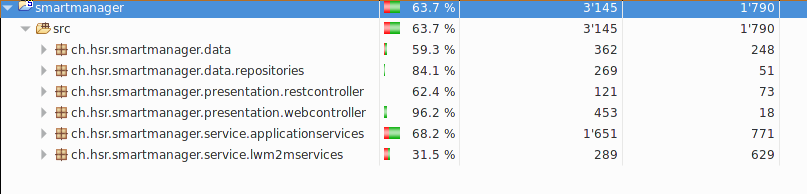
\includegraphics[scale=0.5]{../04_Realisierung/images/testcoverage.png}
\caption{Testabdeckung}
\end{figure}

Durch die durchgeführten Integrationstests wurde eine Testabdeckung von 63.7\% erreicht. Dabei wurden alle relevanten Klassen getestet und Getter- sowie Setter-Methoden ausgelassen.

Es war mit der Testumgebung nicht möglich einen LwM2M-Client zu simulieren. Dadurch konnten alle Methoden, welche auf LwM2M-Clients zugreifen, nicht getestet werden.